\documentclass[xetex,mathserif,serif]{beamer}
\usepackage{beamerstyle}

\usetheme{default}


%\useoutertheme{infolines}
%\useoutertheme{smoothbars}
\useoutertheme{miniframes}

\usecolortheme{seahorse}
%\usecolortheme{seagull}
\useinnertheme{circles}

%\beamertemplatenavigationsymbolsempty

%\setbeamercolor{title}{fg=black!80}
%\setbeamercolor{frametitle}{fg=black!80}
%\setbeamercolor{normal text}{bg=white,fg=black!80}

\title{Μελέτη και υλοποίηση συστήματος αυτοματισμού για την απομακρυσμένη
παρακολούθηση περιβαλλοντικών συνθηκών}

\author{Θεόδωρος Ελευθέριος \textsc{Πάνου}\\ΑΜ 071045}

\institute[ΤΕΙ Αθήνας]{
    Τεχνολογικό Εκπαιδευτικό Ίδρυμα Αθήνας\\
    Σχολή Τεχνολογικών Εφαρμογών\\
    Τμήμα Πληροφορικής
}

\date{Αθήνα 2014}

\begin{document}


\begin{frame}[plain]
    \titlepage
\end{frame}


\begin{frame}
    \frametitle{Περιεχόμενα}
    \tableofcontents
\end{frame}


\section{Γενικά}

%\begin{frame}
%    \begin{center}
%    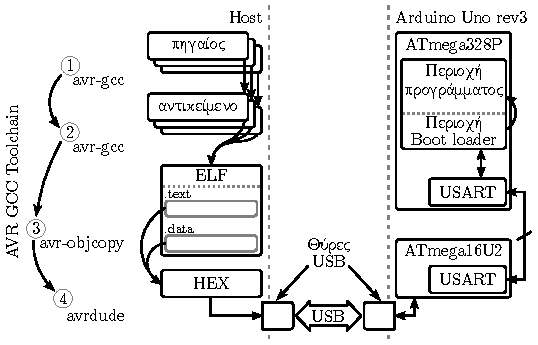
\includegraphics[scale=0.5]{avr_toolchain}
%    \end{center}
%\end{frame}

% arduino


%
%Χρήστης - Συσκευή - Δοχείο
%

\begin{frame}\frametitle
    {Καθήκοντα συσκευής}

    \begin{columns}[T]
    \column{5.5cm}
    \begin{block}
        {Λήψη δεδομένων HTTP}

        \begin{itemize}
        \item Ενεργοποίηση διακομιστή
        \item Τρόπος διασύνδεσης με τρίτους
        \end{itemize}
    \end{block}

    \column{5.5cm}
    \begin{block}
        {Περιοδική αφύπνιση}

        \begin{itemize}
        \item Έλεγχος χρόνου από πρόσφατη μέτρηση
        \item Εκκίνηση νέας εργασίας
        \end{itemize}
    \end{block}
    \end{columns}

    \begin{center}
        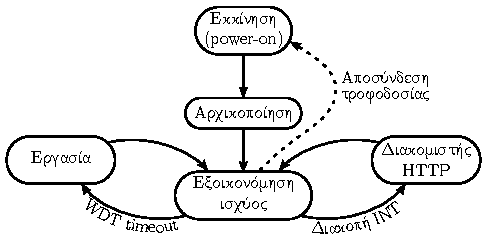
\includegraphics[scale=0.65]{mcu_tasks}
    \end{center}
\end{frame}


\section{Εργασία μέτρησης}

\begin{frame}\frametitle%
    {Κεφαλή αισθητήρων}

    \begin{itemize}
    \item Κινητό εξάρτημα με αισθητήρες
    \item Κινείται επάνω και προς το υλικό (3 άξονες γραμμικής)
    \item Επιτρέπει δειγματοληψία σε τυχαία σημεία
    \item Πολλαπλές μετρήσεις παρέχουν μία ιδέα της κατάστασης
    \end{itemize}

    \begin{center}
    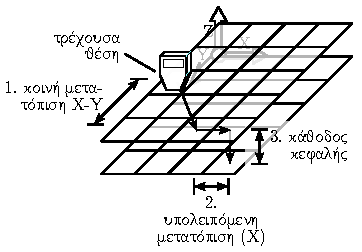
\includegraphics{drive_translation}
    \end{center}
\end{frame}

%    \item Σύστημα συντεταγμένων
%    \item Λειτουργικό εύρος

\begin{frame}\frametitle%
    {Υποσύστημα κίνησης}

    \begin{columns}
    \column{5.5cm}
    \begin{itemize}
        \item Έλεγχος θέσης κεφαλής
        \item Χρήση υλικού αντί CPU
        \begin{itemize}
            \item Παραγωγή και παύση ελέγχου
        \end{itemize}
    \end{itemize}

    \column{5.5cm}
    \begin{itemize}
        \item Προφύλαξη από πρόσκρουση στα άκρα
            \begin{itemize}
            \item Επιστροφή και εκ νέου προσπάθεια
            \end{itemize}
    \end{itemize}
    \end{columns}

    \begin{center}
    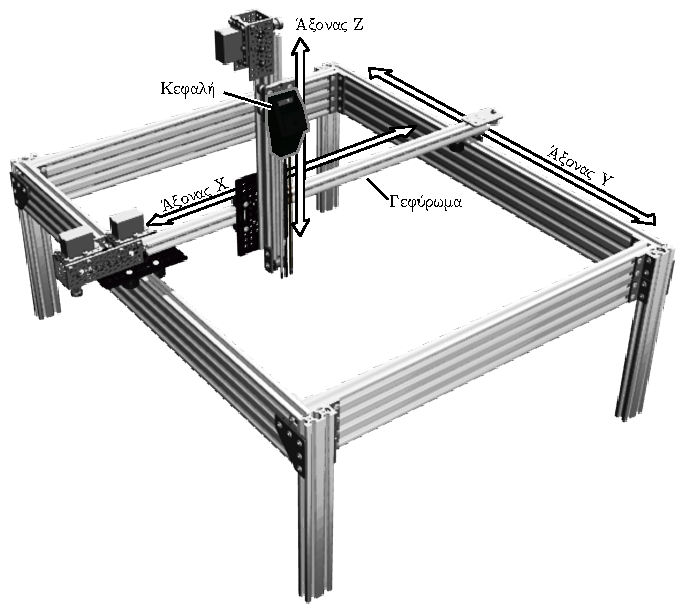
\includegraphics[scale=0.5]{construct_device}
    \end{center}
\end{frame}


\begin{frame}\frametitle
    {dsfsdf}

    \begin{columns}[T]
    \column{5cm}
    \begin{itemize}
    \item Υποδιαίρεση επιφάνειας σε θέσεις 4cm\tsup{2}
    \item Σύστημα συντεταγμένων [X, Y, Z]
    \item Παράλληλη μετατόπιση σε επίπεδο X-Y
    \item Θέση επιστροφής (homing) κατά την έναρξη
    \item Προσαρμογή σε ιδεατές διαστάσεις
    \end{itemize}

    \column{6cm}
    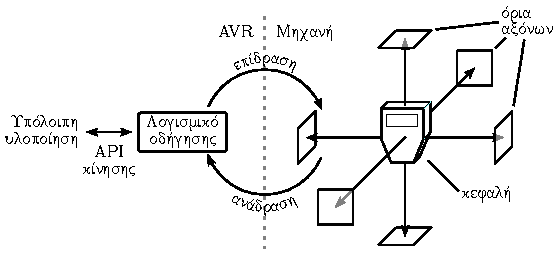
\includegraphics[scale=0.65]{drive_lvl-0}

    \rule{0pt}{0.5cm}

    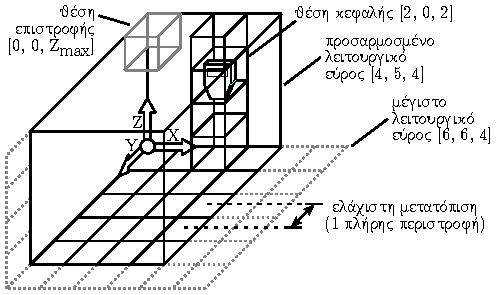
\includegraphics[scale=0.65]{drive_coordinates}
    \end{columns}
\end{frame}


\begin{frame}\frametitle%
    {Κωδικοποιητής κίνησης}

    \begin{columns}[t]
    \column{5.5cm}
    \begin{itemize}
        \item Παραγωγή παλμών από περιστροφή κινητήρα
        \item Αυτοσχέδιος με χρήση ανακλαστικού αισθητήρα
        \item Προσαυξητικός
    \end{itemize}

    \column{5.5cm}
    \begin{itemize}
        \item Ενεργοποιείται μόνο όσο λειτουργεί ο κινητήρας
        \item Ένας για κάθε άξονα κίνησης
    \end{itemize}
    \end{columns}

    \begin{columns}
    \column{5.5cm}
    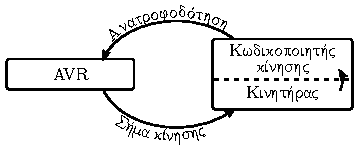
\includegraphics[scale=0.65]{encoder_lvl-0}
    \column{5.5cm}
    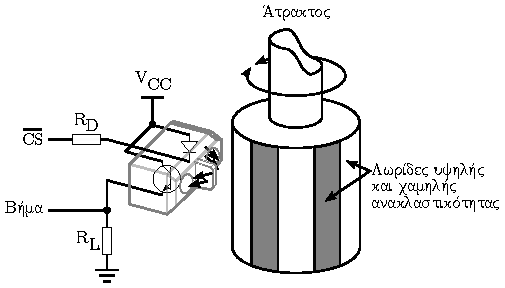
\includegraphics[scale=0.65]{encoder_lvl-1}
    \end{columns}
\end{frame}

% PWM

%\begin{frame}%\frametitle
%%    {}

%    \begin{center}
%    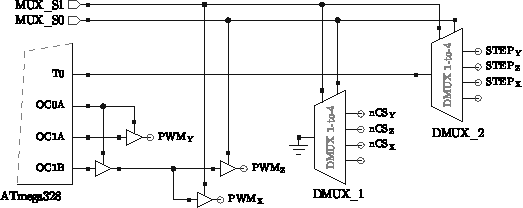
\includegraphics{drive_schem_step-and-pwm}
%    \end{center}
%\end{frame}


\begin{frame}\frametitle
    {Το υποσύστημα κίνησης συνολικά}

    \begin{center}
    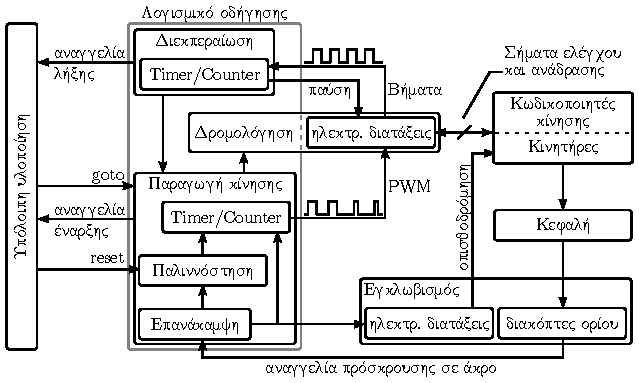
\includegraphics[scale=1]{drive_lvl-1}
    \end{center}
\end{frame}


\begin{frame}
    \frametitle{Κύκλος μετρήσεων}
    \begin{itemize}
%--    Υπολογισμός χρόνου μεταξύ πρόσφατης μέτρησης και τρέχουσας ώρας ~~
%    Κύκλοι μετρήσεων (goto-sample) % Implies asynchronous
%    Ασύγχρονη υλοποίηση / Σταδιακή ολοκλήρωση
    
    \item Καθορισμός νέας θέσης
    \item Ανάγνωση αισθητήρων
    \item Εκτίμηση χρόνου ολοκλήρωσης
    \item Καταχώρηση σε ημερολόγιο
    \end{itemize}

    \begin{center}
        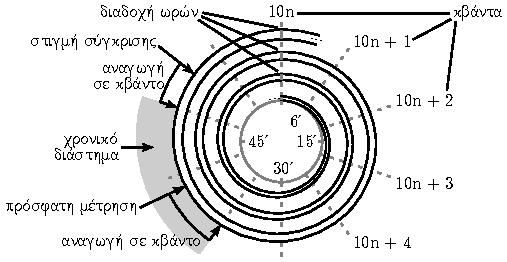
\includegraphics[scale=0.65]{task_interval}
        \hfill
        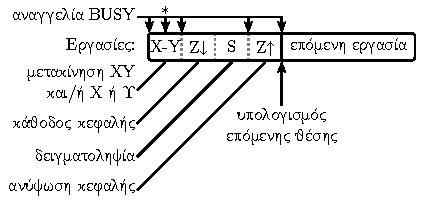
\includegraphics[scale=0.65]{task_estimate-update}
    \end{center}
%[hints drivesystem]
%[needs RTC]
\end{frame}


\begin{frame}
    \frametitle{Ημερολόγιο}
    \begin{itemize}
    \item Διαχείριση εγγραφών μετρήσεων
    \item Διατήρηση πιο πρόσφατων μετρήσεων
        \begin{itemize}
        \item Κυκλική μνήμη (μείωση επανεγγραφών)
        \item Δυαδική αναζήτηση (μείωση αναγνώσεων)
        \end{itemize}
    \item Εικονικά σετ εγγραφών
        \begin{itemize}
            \item Διευκόλυνση σελιδοποίησης
        \end{itemize}
    \end{itemize}
    \begin{center}
        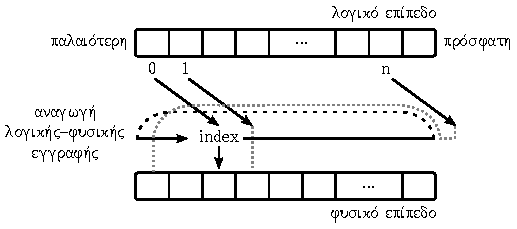
\includegraphics[scale=0.65]{log_structure}
    \end{center}
\end{frame}
%    (Δομή εγγραφής· implies BCD)


\begin{frame}\frametitle
    {Διαστρωμάτωση κεντρικών μονάδων S\slash{}W και H\slash{}W}

    \begin{center}
    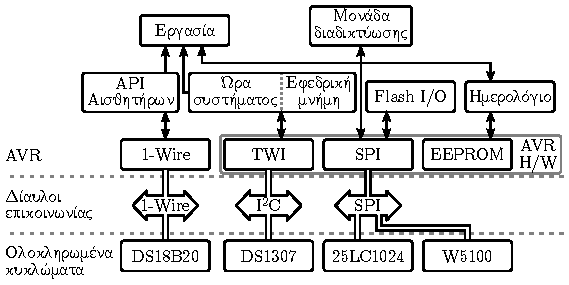
\includegraphics[scale=1]{foundation_lvl-0}
    \end{center}
\end{frame}






\section{Διεπαφή επικοινωνίας}

\begin{frame}
    \begin{center}
    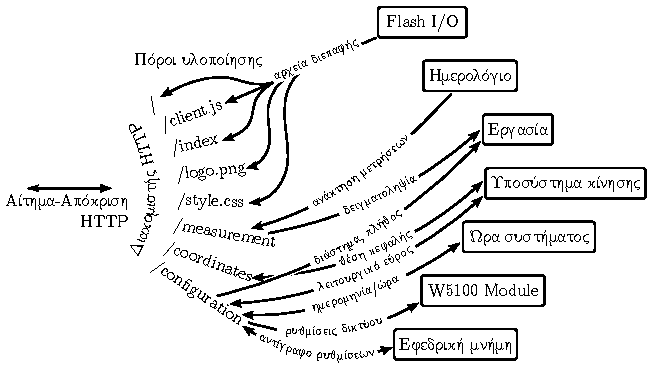
\includegraphics{network_resources}
    \end{center}
\end{frame}

\begin{frame}
    \begin{center}
    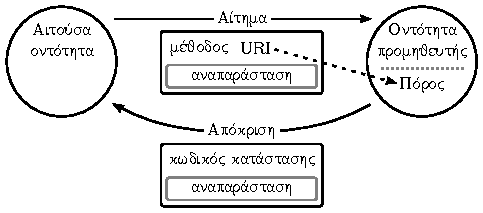
\includegraphics[scale=0.5]{network_requester-provider}
    \end{center}
\end{frame}

\begin{frame}
    \begin{center}
    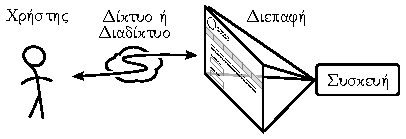
\includegraphics[scale=0.5]{network_interface-0}
    \end{center}
\end{frame}


\begin{frame}
    \begin{center}
    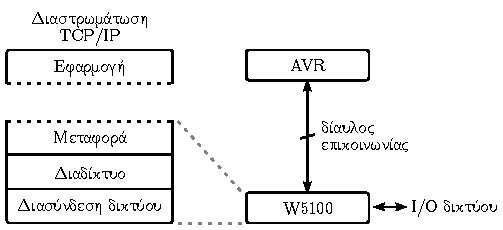
\includegraphics[scale=0.5]{network_lvl-0}
    \end{center}
\end{frame}

\begin{frame}
    \begin{center}
    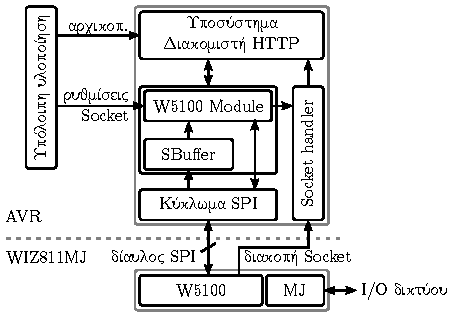
\includegraphics[scale=0.5]{network_lvl-1}
    \end{center}
\end{frame}

%Αίτημα - Απόκριση HTTP
%    


%Διακομιστής HTTP
%    Ανάλυση επικεφαλίδων
%    Προώθηση σε ρουτίνα περάτωσης

%[κάποια πράγματα για HTTP]

% Εργοστασιακές ρυθμίσεις
% Δίαυλοι επικοινωνίας

%\section{Εισαγωγή}


%\section{Μετρήσεις}

%\section{Υποσύστημα κίνησης}
%\subsection{Κεφαλή}
%\subsection{Συντεταγμένες}

%\section{Επικοινωνία με συσκευή}

%\begin{frame}
%\frametitle{Υποσύστημα κίνησης}
%\begin{itemize}
%    \item Διακριτές θέσεις κεφαλής
%    \item Ανεξαρτησία από CPU (κίνηση, ολοκλήρωση)
%    \item Ανασταλτικοί διακόπτες
%    \item Επαναφορά και επανάκαμψη
%    \item Θέση επιστροφής (homing)
%    \item Λειτουργία σε προσαρμοσμένες διαστάσεις
%\end{itemize}
%    \vfill
%    \begin{center}
%        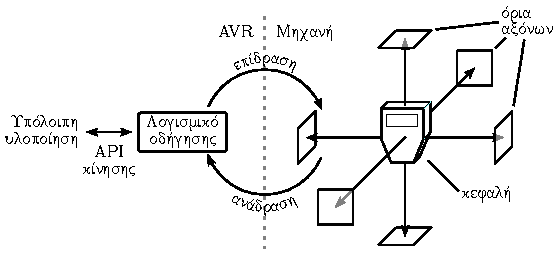
\includegraphics[scale=0.65]{drive_lvl-0}
%%        \hfill
%%        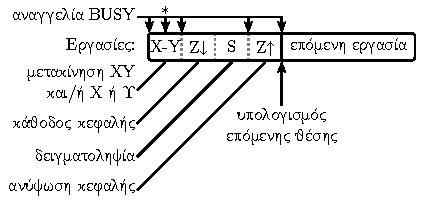
\includegraphics[scale=0.65]{task_estimate-update}
%    \end{center}
%\end{frame}

%\begin{frame}
%\frametitle{Εργασία μετρήσεων}
%\begin{itemize}
%    \item Περιοδική αφύπνιση (από WDT)
%    \item Εκκίνηση κύκλου μετρήσεων (εργασία)
%    \item Καταχώρηση σε ημερολόγιο μετρήσεων
%    \item Εκτίμηση χρόνου ολοκλήρωσης
%\end{itemize}
%    \vfill
%    \begin{center}
%        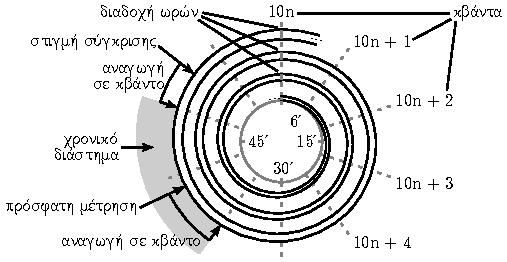
\includegraphics[scale=0.65]{task_interval}
%        \hfill
%        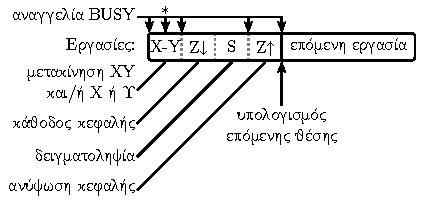
\includegraphics[scale=0.65]{task_estimate-update}
%    \end{center}
%\end{frame}

\begin{frame}
\end{frame}

\end{document}
